\section[Related Work]{Related Work}
\label{sec:Related Work}

Several research works have been conducted regarding the use of games for teaching computer programming and software engineering.

The chapter illustrates the related research work as well as the related games that were developed for Game-Based Learning in SE.

\subsection{Game-Based Learning research in SE}
The following is an overview of the previous work regarding Game-Based Learning in the field of software engineering.

Tao et al. \cite{educational} emphasize learning software engineering through different gaming approaches. In their research, they found that gaming for software engineering education required a slightly different approach than the traditional Game-Based Learning methodologies. They created Pex4Fun to serve both the social aspects of Game-Based Learning and the presentation of software engineering content. The learning outcome from the research work is gaming and entertainment can be a source of education and that interactive learning has excellent value. Another discovery is that learning while playing can be effective in the industrial field.

Swapneel et al. \cite{halo} discussed how highly addictive socially optimized (HALO) provides concentration through an adaptive environment. The game environment is developed in such a way so that the player can enjoy the work in a gaming atmosphere. 
it for company uses. The initial stage is known as ‘Quest’, which is a preliminary introduction of the system. Here someone senior must work voluntarily or can be assigned. If the quest is harder for a single player, it could be done in a team, and then it is called a party. A simple quest can form a chain of quests, like use-cases or bug fixing. Another essential aspect is context switching. If an employer works on different modules then it will require more time, but HALO groups the same type of coding all together so that less context switching is required. In this process, a balanced environment has been created where players progress through multiple difficulties. The game is designed as a simple plugin to integrate with an IDE\footnote{Integrated Development Environment (IDE) is known as a software application that provides comprehensive facilities to computer programmers for software development.}, such as Eclipse or Microsoft Visual Studio. Making the user comfortable with the working environment is one of the significant contributions of HALO. A gamer is more comfortable in the gaming environment using this technique HALO adopted a context switching free environment. HALO is designed for the software industry, where the different projects have different requirements. Along with that is supports various social aspects like teamwork, project management.
Both the academic and industrial fields can be beneficial by adopting the game-based approach in software engineering.  Evaluation of the technique was not present, which is one of the drawbacks of this research.  

Miljanovic et al. \cite{robobug} discussed Robobug, a debugging technique through gaming in their research paper. Debugging is an essential tool in programming. Many good programmers struggle to find the bugs in a code segment. Debugging requires practice and patience; both might be difficult for a new programmer. Many computer science students struggle with debugging and feel left behind. Robobug presents different debugging techniques at different levels. It also has hints, which are very helpful for learning.

Szabo \cite{gamedev} proposed GameDevTycoon for teaching software engineering. Based on their work, there are thirteen different criteria for Game-Based Learning. GameDevTycoon covers most of the criteria. Gameplay analysis and software process models are simultaneously covered in the game. Three primary stages of software development are taught through the gameplay. The initial stage is known as the garage, the second stage is called team management, and the final stage is known as world domination. Each stage has separate responsibilities; for example, in the initial stage in software development, one should focus on the quality and latest research. As the project grows, team building is an additional responsibility that needs to be handled. When the project is in the saturation stage, new research works should be promoted so that the new technology can be cultivated. Again some small but significant issues regarding team bonding and employee workload also need to be adequately addressed in terms of good team bonding.

Pieper et al. \cite{SEMAT} presented a case study of the Software Engineering Method and Theory (SEMAT) to identify the educational outcomes in Digital Game-Based Learning. SEMAT is a part of the emerging OMG\footnote{The Object Management Group (OMG) is a computer industry standards consortium.} standard \cite{kernerl}. The case study shows that the evaluation of a developed integrated scenario can provide an in-depth analysis of the result. Nevertheless, the data was not sufficient to reach a conclusive decision regarding the pattern of learning. As a result, SEMAT was not referred to as a standard. The researchers state that if the study could be conducted in a broader spectrum (larger dataset), the result of the case study might be eligible for a conclusive outcome.

Mauricio et al. \cite{gamesforlearning} identified a different methodology that can be or is already applied in different interactive games for Software Engineering (SE) Game-Based Learning. Also, they explored different primary studies related to SE education, found the learning outcomes and mapped those outcomes to different SE project stages. 

Vladimir et al. \cite{gamification} discussed the different classifications of gameplay and their impact on several learning criteria. According to the researchers, gamification is a growing area in the business industry. The researchers emphasized the SWOT (Strengths, Weaknesses, Opportunities, Threats) framework \cite{swot} to find the learning criteria. However, they found that creating a software engineering Game-Based engine is a challenging task, one which programmers and industry should give a high priority. 

\subsection{Games for Learning Software Engineering}
Several games have been created for teaching the basics of programming. However, most of them are platform-oriented (i.e. only work on Windows) or target a specific programming language (e.g. C++ or Java). For learning the basics regarding computer programming, it is essential to understand the underlying logic and conceptual ideas. In this section, several types of games, especially board games, card games, desktop-based games and web-based games, are presented.

\subsubsection{Board Games}
Board games are a part of tabletop games where different components of the game can be moved on an adjacent surface or board according to some predefined rules \cite{boardgames}. The following are a couple of board games, which teach different aspects of computer programming.

Battle Bots v2 \cite{BattleBotsv2}  was inspired by the Robo Rally \cite{roborally} game. The required number of players for the game is between two and twenty. In the middle of the board, there is a repair center. Each player will start the game with twenty-two cards. Each move is divided into two groups: the programming round and the action round. In the programming round, players have to play the movement cards. In this stage, no action card can be played. In action round, there are five-phase where different action cards can be played along with movement cards. The player who survives the match wins the game. The main advantage of the game is that the players have to plan about the moves, which is an important programming concept, as in programming, it is essential to set the goal. A player can design his/her game plan depending on the other players’ moves or personal requirements. As a result, a fair amount of calculation is needed, which is very important in the logical aspect of computer programming. The game has no actual programming interface, which is one of the drawbacks of the game. 

Robot Turtles \cite{RobotTurtles} is a game to teach kids to code by using simple direction cards to move a specific coloured turtle. The main focus of the game is to get the coloured turtle to the same coloured jewel piece on the board. There are three instructions: forwards, rotate 90 degrees left and rotate 90 degrees right. There are also some obstacles where players might have to use different techniques to overcome the situation, and some unique cards are also introduced like fire cards for shooting. The higher the level, the more complex cards need to be used.
Regarding programming, the jump card is the most crucial one. The idea of jump cards is that they can be replaced with a set of instruction cards that can be used repeatedly. There is also a bug card that can undo the immediate move the player has made. Robot Turtles is designed for kids’ initial steps in programming, like single statement compilation, which is well executed through a single card movement. The introduction of a jump card is an excellent initial concept of function calls. Bug cards introduce the idea of mistakes in programs.

Code Master \cite{CodeMaster} is a single person puzzle game that teaches logical problem-solving. There are sixty levels in the game with several challenging levels. The game consists of a map that has six different levels ranging from easy (green) to expert (red). There is also a guide scroll that indicates the order in which the program statements should run. Also, the guide has places for conditional tokens. There are three colours: green, blue and red. For each path, there is a specific token related to the colours. Numerical numbers are represented in the map nodes. The goal is to get to a portal and collect crystals using a limited path and moves. The game focuses on the programming construct of conditional statements (i.e. if-else). Some nodes have a self-loop, which illustrates the concept of a repeat statement. Finally, the shortest path selection is also a focus point. The game requires essential thinking before each move, which is vital for developing logical thinking. Unidirectional and bi-directional edges in a graph can be learned by playing the game. 

\subsubsection{Card Games}

A card game can be defined as a game that involves different playing cards as the main components with which the game can be played \cite{cardgames}.

Potato Pirates \cite{PotatoPirates} was the only physical card game found that intends to teach programming concepts. The main objective of the game is to make the user familiar with different programming concepts through social interactions. The final goal of the game is to achieve seven specific cards, named Potato King, through different logical actions performed through different cards. To win the game, a player needs to eliminate all the other ships in possession of the other players or acquire all seven Potato Kings by drawing them from the deck or by eliminating other players’ ships and seizing their cards. Players can power up their attacks with programming concepts cards such as loops and conditionals. The game covers the concepts of programmings such as variables, functions, while-loops, if-else conditionals and nested-loops. Some surprise cards serve the purpose of interrupts and control flow. The game illustrates the branching condition very nicely, which is equivalent to the if-else statement. The use of variables is well defined. Different repeat structures are also presented in a reasonable manner such that the game covers the loop structure of programming languages. There is also an option for creating a loop inside a loop, which is known as a nested loop. The game also covers the case structure (switch case or nested if-else).

\subsubsection{Web-based Games}

Games that can be played on the World Wide Web are known as web-based games. These games use standard web technologies or browser plugins \cite{webbasedgames}.

CodeCombat \cite{CodeCombat} is a web-based game focusing on learning JavaScript, Python, and other programming languages. The game is built upon concepts of swords-and-sorcery where the player has to role-play as a warrior. The main objective of the game is to learn necessary programming skills by overcoming different challenges like clearing the maze, picking up gems and avoiding any spikes or attacking ogres. The gameplay is split between a code editor on the right and a simulation effect on the left. Figure \ref{fig:CodeCombat} shows the interface of the game. The avatar is controlled by using a set of commands.  In each level, the player has to accomplish a set of tasks. As the game progresses, the player is gradually introduced to new concepts like loops, conditionals, and variables. If a person does not have programming experience, CodeCombat is very suitable. As the game progresses, the tasks involve more complex programming concepts. Most importantly, the levels themselves become more complicated due to possible interactions with the objects in the game world.\\

\begin{figure}[ht!]
	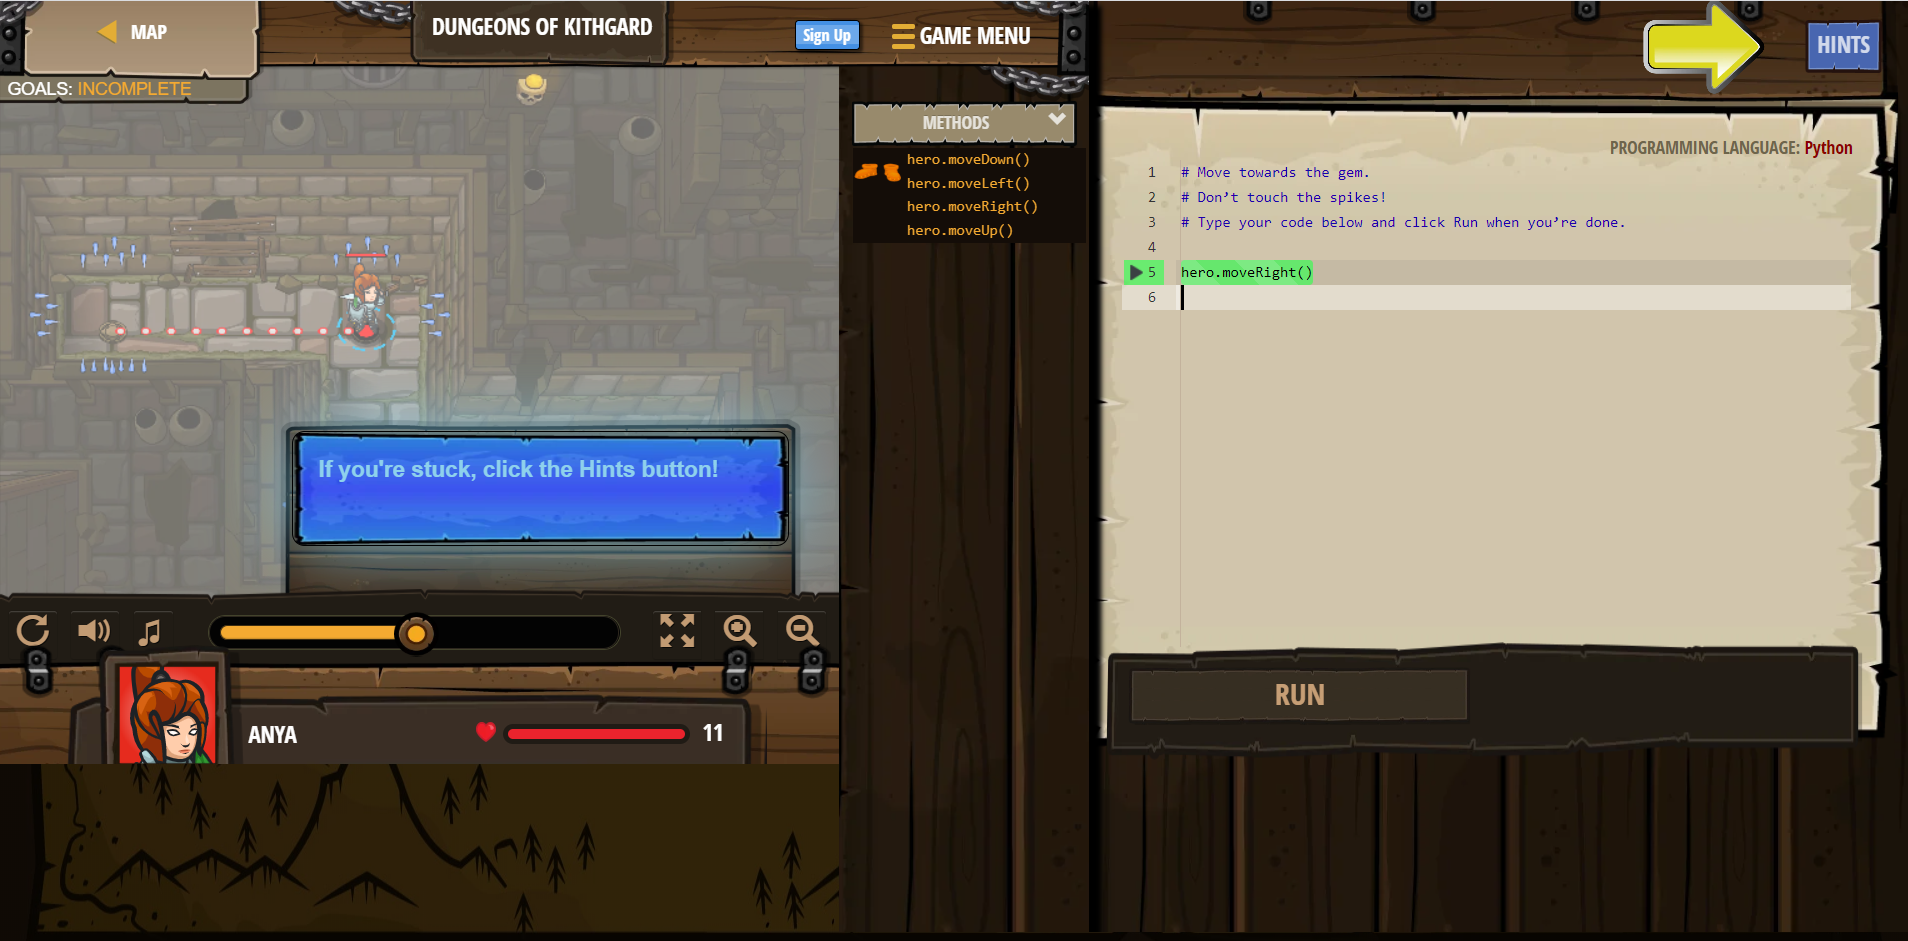
\includegraphics[width=\columnwidth]{images/CodeCombat.PNG}
    \caption{CodeCombat gameplay}
    \label{fig:CodeCombat}
\end{figure}

Blocky maze \cite{Blocklymaze} is a game that introduces the concept of programming loops and conditions in Javascript without writing any Javascript code. The game is a combination of levels that teach programming. It is designed for children who have not had prior experience with computer programming. The game uses a graphical programming language implemented in JavaScript, which can compile to JavaScript, Dart or Python. In the game, programming is done by dragging and dropping code blocks onto a design surface. Figure \ref{fig:BlocklyMaze} shows the interface of the game. The main objective of the game is to take the avatar from a starting point to the endpoint. There are a total of ten levels, and the complexity increases as the game progress. Some goals are set to solve the maze in a particular number of steps, which is also challenging. The game interface is similar to a Google Map, which might help the user to adopt the game. 

\begin{figure}[ht!]
	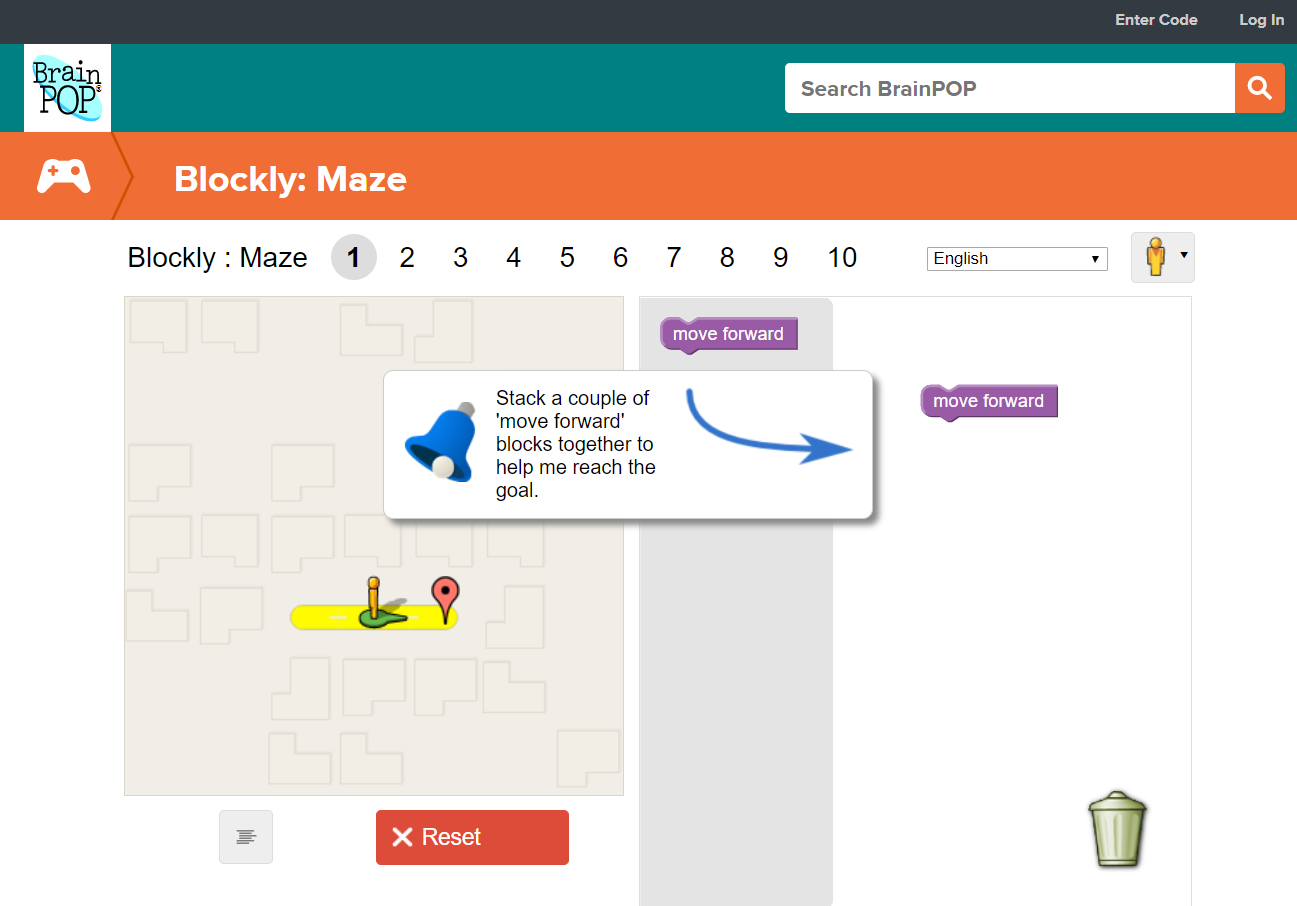
\includegraphics[width=\columnwidth]{images/BlocklyMaze.PNG}
    \caption{Blockly Maze gameplay}
    \label{fig:BlocklyMaze}
\end{figure}

CodinGame \cite{Codingame} supports many programming languages. The main objective of the game is to improve players’ coding skills by solving different problems, applying new strategies and getting inspired by other strong opponents. The game can be played in single and multiplayer mode, which gives it the feeling of fun rather than learning. A player can choose any programming language among more than twenty, such as Python, Ruby, Java, and Scala. The targeted group for the game is the people who have basic programming knowledge as well as expert developers. In the game, users create a profile, which is used for challenges and contests. There are opportunities for players to make their profile public so that employers can find them to offer them a job. Also, the game has a forum for members to chat about languages, questions, and share information. The game is not for beginners because it requires some basic knowledge of programming. Figure \ref{fig:CodinGame} shows the interface of the game.

\begin{figure}[ht!]
	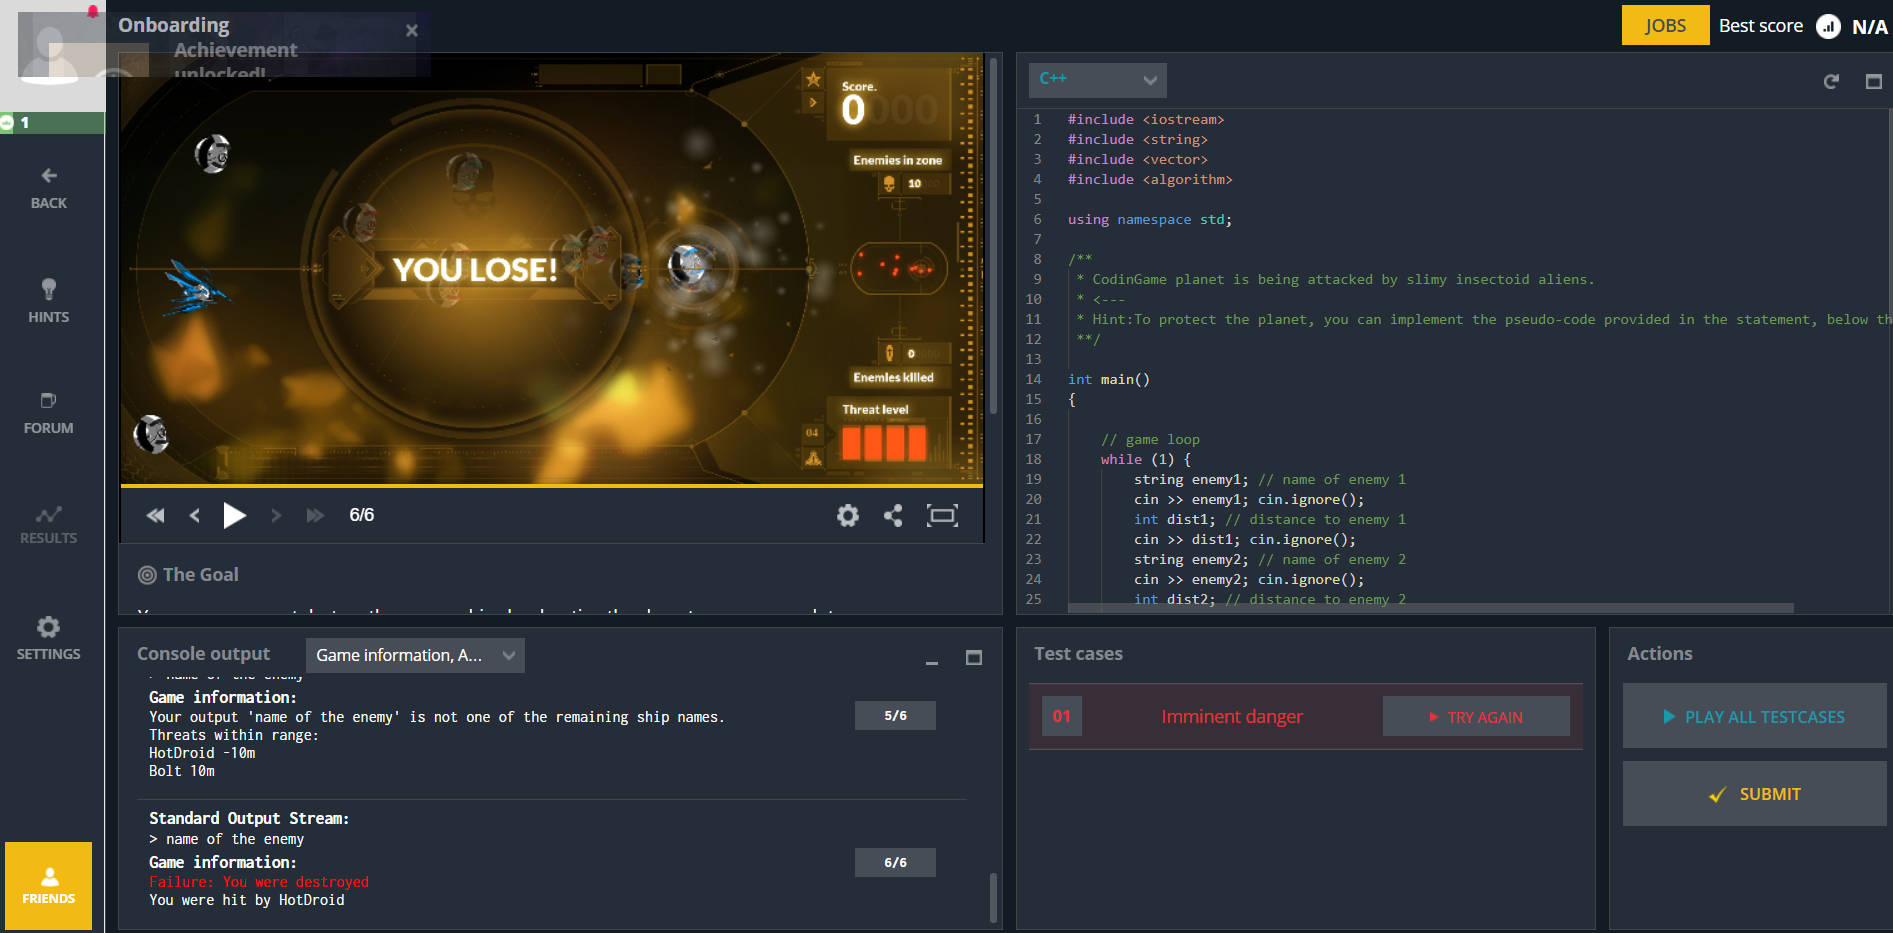
\includegraphics[width=\columnwidth]{images/CodinGame.PNG}
    \caption{CodinGame gameplay}
    \label{fig:CodinGame}
\end{figure}

\begin{figure}[hbt!]
  	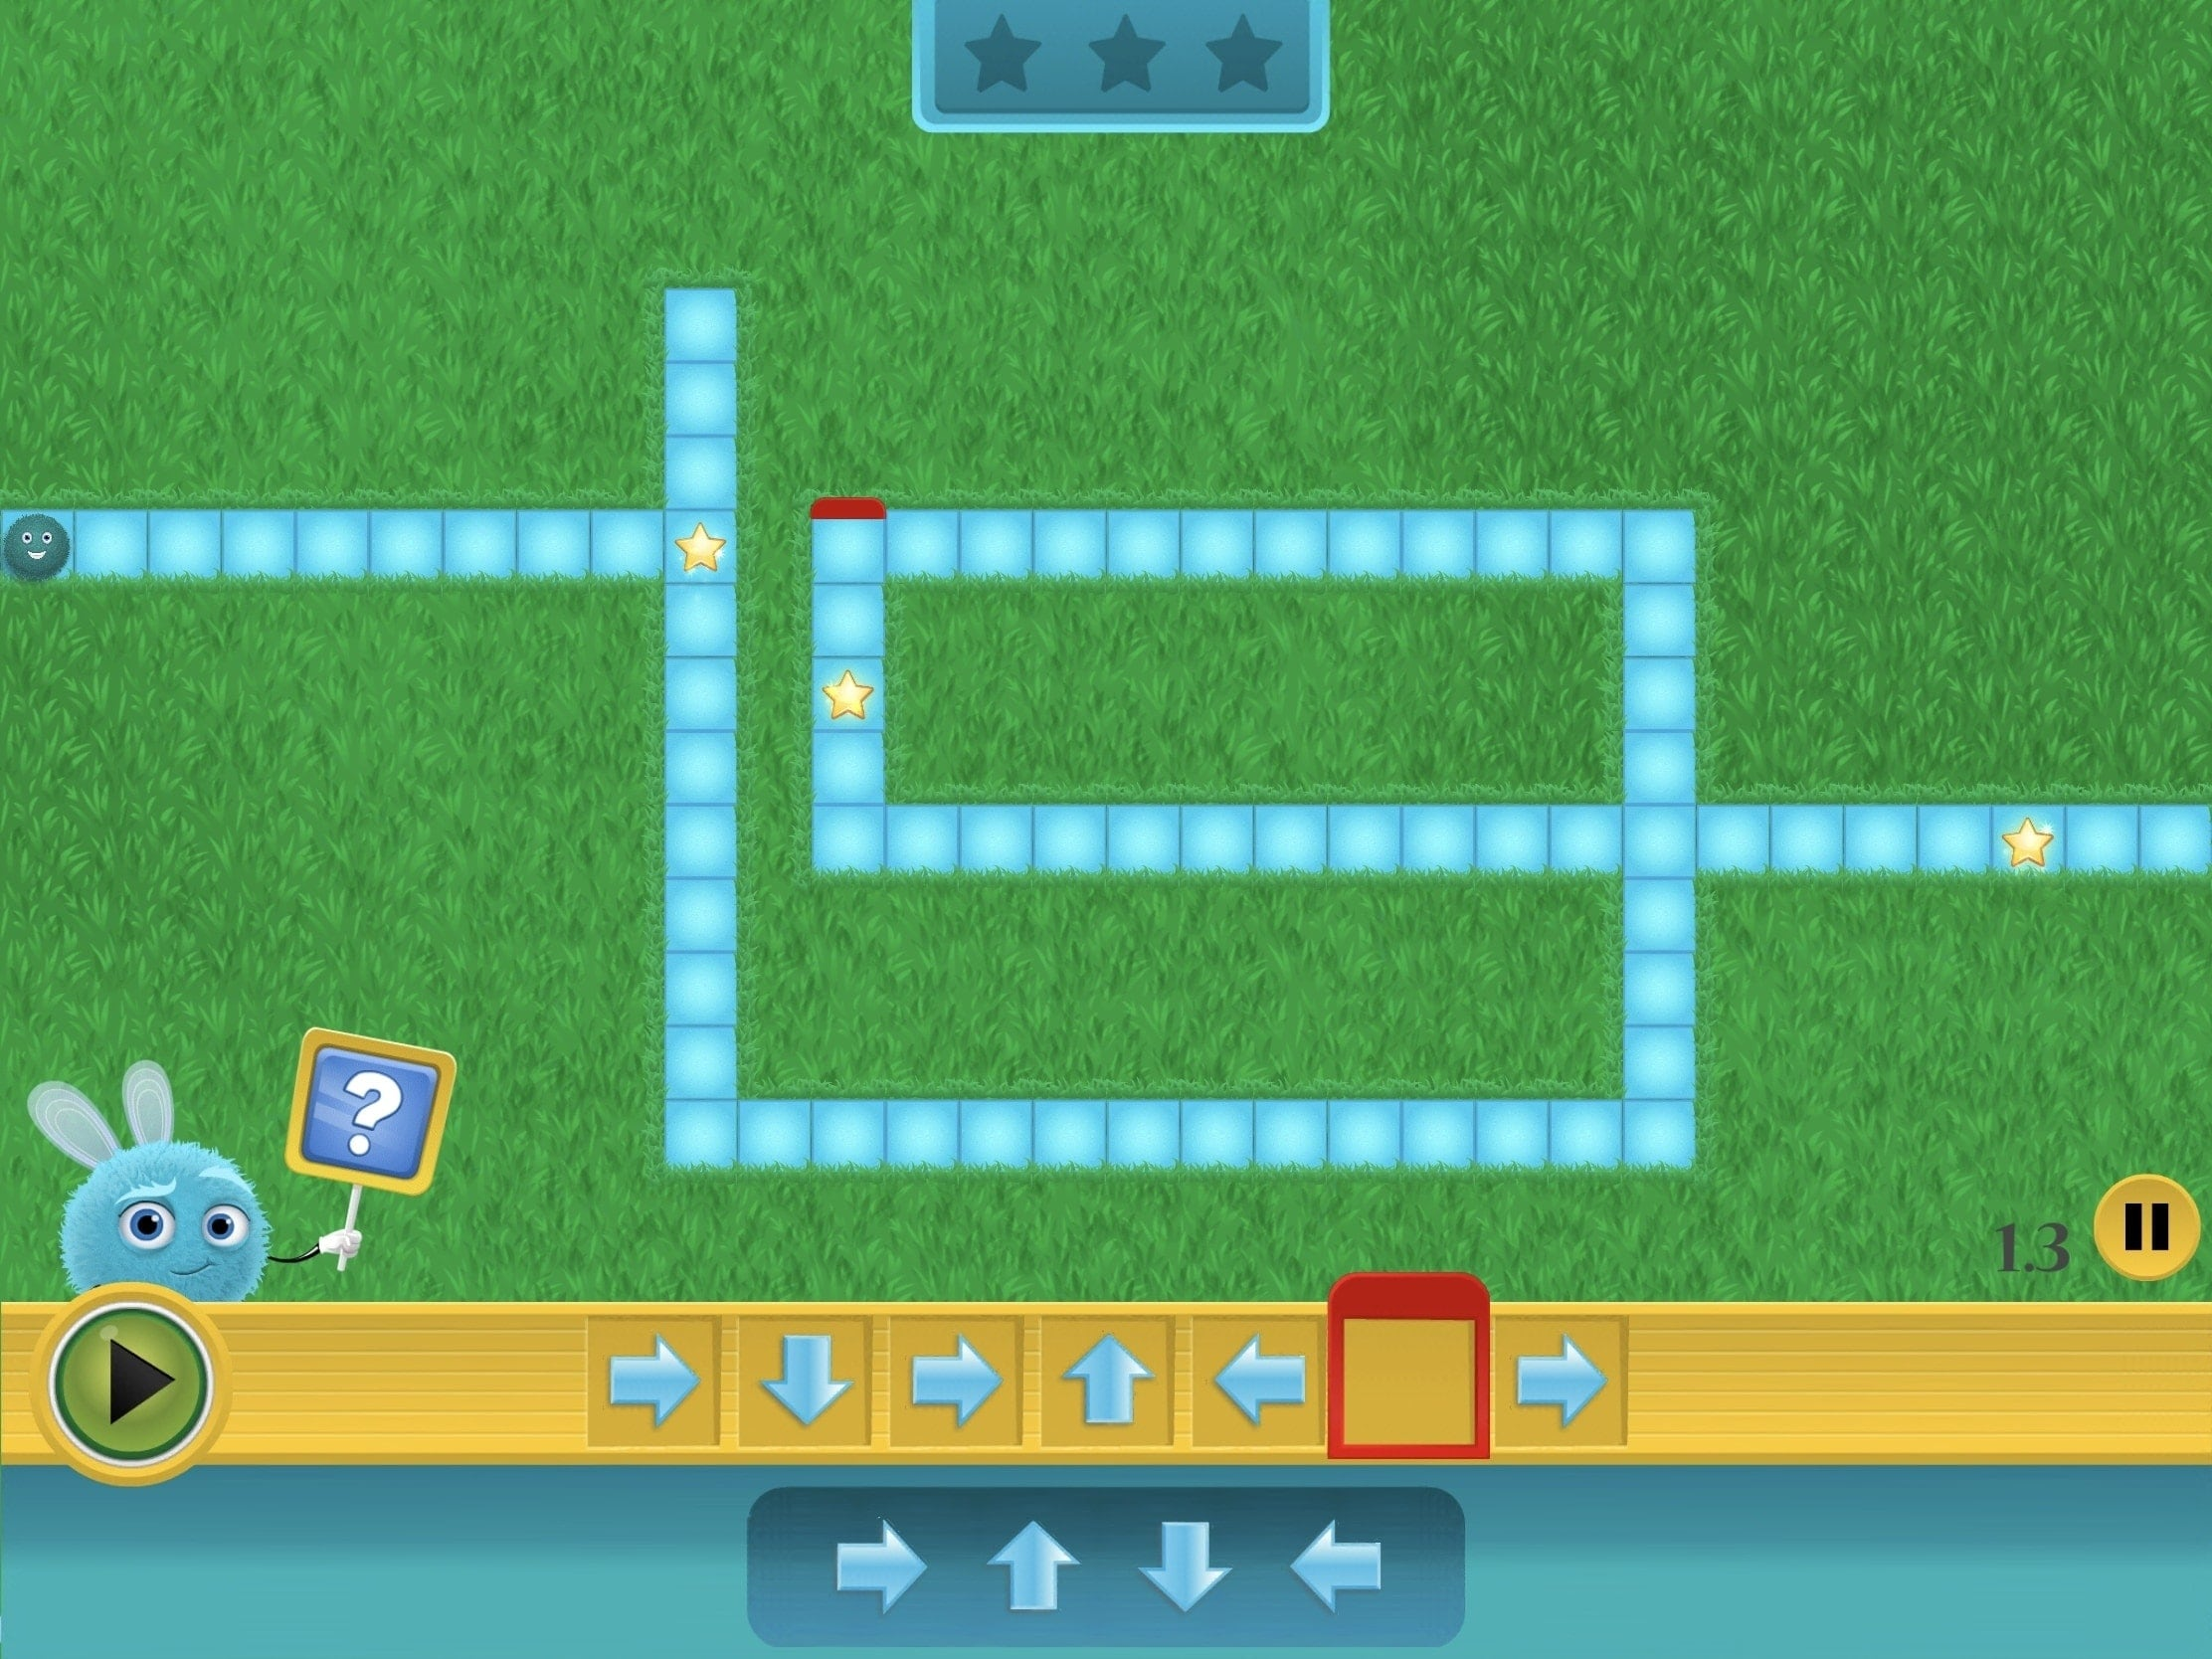
\includegraphics[width=\columnwidth]{images/Kodable.PNG}
    \caption{Kodable gameplay}
    \label{fig:Kodable}
\end{figure}

Kodable \cite{Kodable} is a game developed for kids that focuses on introducing logic and the decisions (i.e. if-then-else) in computer programming. Kodable’s programming language introduces players to step-by-step statements with different instructions using in the programming language. The primary programming concepts of conditional statements and loop structure, is well defined in the game. The social aspect of the game is presented into a parents section with written teaching instructions that assist the parent to unlock different levels for kids and extend logic skills into real life. The game is comprised of many features that are appropriate for children. The activities in the game help the player to think like a programmer, solve different problems and eventually to writing real code using the game’s custom coding interface. Figure \ref{fig:Kodable} shows the interface of the game. For logic development, the game focus on learning the importance of statement sequence. The game introduces kids to different types of data, such as integers and strings, and data structures, such as arrays. Finally, object-oriented programming concepts are also introduced by the game. 


Program Wars \cite{ProgramWars} is a web-based card game. The game focuses on learning programming and cybersecurity concepts. The player’s objective is to achieve a specific number of points through different cards. The game is platform-independent, which means that it is not focused on any single programming language. Instead, the game helps to develop an understanding of the underlying logic of programming. Here the players do not have to be concerned about syntax errors, and programming terms are being described using an elementary vocabulary. In Chapter \ref{ch:Overview of Program Wars}, a more detailed analysis regarding Program Wars is presented.   

%\section{Summary}
%Based on the related research works examined, practical implementation (i.e. learning a real programming language) and visualization of program results are essential in software engineering education. Also, learning through gameplay has more sustainable effects\cite{effectivenessofgames}. The main challenge of Game-Based Learning for software engineering is to maintain a balance between learning and engagement \cite{educationalgamedesign}. The gameplay should be presented in a structured way such that the user can relate the outcome to real-world programming. Most of the research deals with a specific part of a software engineering like debugging, the user interface, and project management.